\documentclass[tikz,border=10pt]{standalone}
% Shared look for every TikZ diagram. Load with % Shared look for every TikZ diagram. Load with % Shared look for every TikZ diagram. Load with \input{../../tools/tikz-style.tex}
\usepackage[T1]{fontenc}
\usepackage{lmodern}
\renewcommand{\sfdefault}{lmr}  % diagrams use the same serif as the text
\usetikzlibrary{arrows.meta, positioning, shapes.geometric, calc, fit, backgrounds}
\definecolor{cblue}{HTML}{4C78A8}
\definecolor{corange}{HTML}{F58518}
\definecolor{cgreen}{HTML}{54A24B}
\definecolor{cred}{HTML}{E45756}
\definecolor{cpurple}{HTML}{B279A2}
\definecolor{cgrey}{HTML}{6B6B6B}
\tikzset{
  every picture/.style={font=\sffamily, line width=1.2pt},
  box/.style={draw=#1, fill=#1!12, rounded corners=4pt, align=center, inner sep=7pt, minimum height=1.1cm},
  box/.default=cgrey,
  arrow/.style={-{Stealth[length=3mm]}, draw=cgrey, line width=1.4pt},
  title/.style={font=\sffamily\bfseries\Large},
  note/.style={font=\sffamily\small, text=cgrey, align=center},
}
\AtBeginDocument{\hyphenpenalty=10000 \exhyphenpenalty=10000}

\usepackage[T1]{fontenc}
\usepackage{lmodern}
\renewcommand{\sfdefault}{lmr}  % diagrams use the same serif as the text
\usetikzlibrary{arrows.meta, positioning, shapes.geometric, calc, fit, backgrounds}
\definecolor{cblue}{HTML}{4C78A8}
\definecolor{corange}{HTML}{F58518}
\definecolor{cgreen}{HTML}{54A24B}
\definecolor{cred}{HTML}{E45756}
\definecolor{cpurple}{HTML}{B279A2}
\definecolor{cgrey}{HTML}{6B6B6B}
\tikzset{
  every picture/.style={font=\sffamily, line width=1.2pt},
  box/.style={draw=#1, fill=#1!12, rounded corners=4pt, align=center, inner sep=7pt, minimum height=1.1cm},
  box/.default=cgrey,
  arrow/.style={-{Stealth[length=3mm]}, draw=cgrey, line width=1.4pt},
  title/.style={font=\sffamily\bfseries\Large},
  note/.style={font=\sffamily\small, text=cgrey, align=center},
}
\AtBeginDocument{\hyphenpenalty=10000 \exhyphenpenalty=10000}

\usepackage[T1]{fontenc}
\usepackage{lmodern}
\renewcommand{\sfdefault}{lmr}  % diagrams use the same serif as the text
\usetikzlibrary{arrows.meta, positioning, shapes.geometric, calc, fit, backgrounds}
\definecolor{cblue}{HTML}{4C78A8}
\definecolor{corange}{HTML}{F58518}
\definecolor{cgreen}{HTML}{54A24B}
\definecolor{cred}{HTML}{E45756}
\definecolor{cpurple}{HTML}{B279A2}
\definecolor{cgrey}{HTML}{6B6B6B}
\tikzset{
  every picture/.style={font=\sffamily, line width=1.2pt},
  box/.style={draw=#1, fill=#1!12, rounded corners=4pt, align=center, inner sep=7pt, minimum height=1.1cm},
  box/.default=cgrey,
  arrow/.style={-{Stealth[length=3mm]}, draw=cgrey, line width=1.4pt},
  title/.style={font=\sffamily\bfseries\Large},
  note/.style={font=\sffamily\small, text=cgrey, align=center},
}
\AtBeginDocument{\hyphenpenalty=10000 \exhyphenpenalty=10000}

\begin{document}
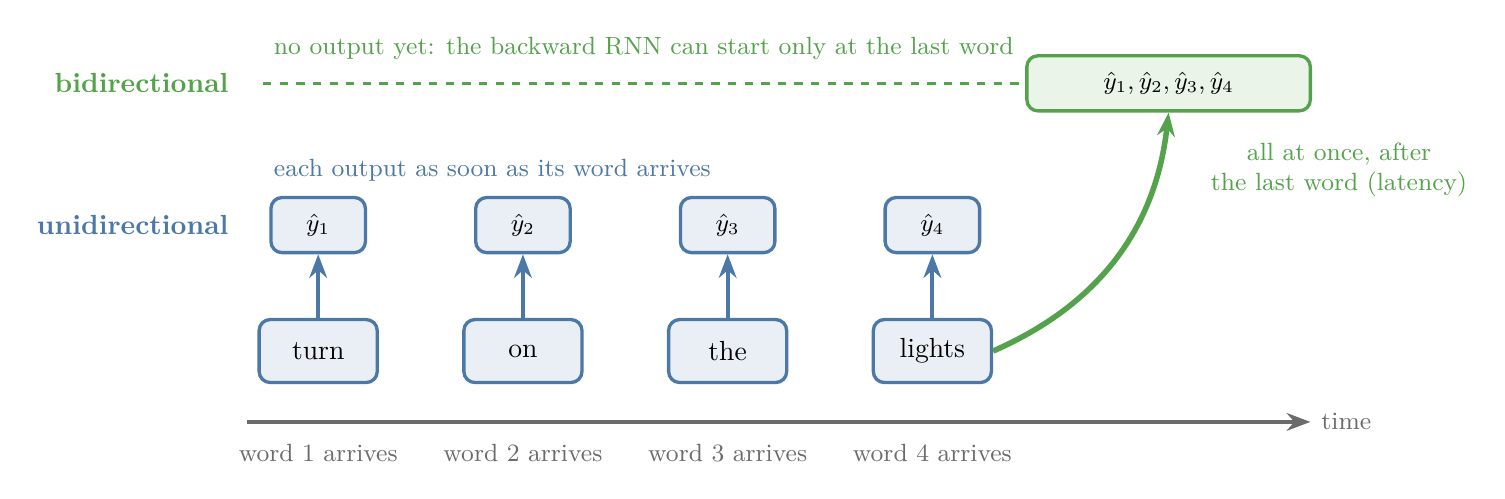
\begin{tikzpicture}[w/.style={box=cblue, inner sep=4pt, minimum height=0.8cm, minimum width=1.5cm, font=\sffamily},
  o/.style={box=#1, inner sep=3pt, minimum height=0.7cm, minimum width=1.2cm, font=\sffamily\small}]
  \draw[arrow] (-0.9,-0.9) -- (12.6,-0.9) node[right, note] {time};
  \foreach \t/\x [count=\i] in {turn/0, on/2.6, the/5.2, lights/7.8} {
    \node[w] (w\i) at (\x,0) {\t};
    \node[note] at (\x,-1.3) {word \i\ arrives};
    \node[o=cblue] (u\i) at (\x,1.6) {$\hat y_\i$};
    \draw[arrow, draw=cblue] (w\i) -- (u\i);
  }
  \node[anchor=east, font=\sffamily\bfseries, text=cblue] at (-1.0,1.6) {unidirectional};
  \node[anchor=east, font=\sffamily\bfseries, text=cgreen] at (-1.0,3.4) {bidirectional};
  \node[note, text=cblue, anchor=west] at (-0.7,2.3) {each output as soon as its word arrives};
  \node[o=cgreen, minimum width=3.6cm] (bo) at (10.8,3.4) {$\hat y_1, \hat y_2, \hat y_3, \hat y_4$};
  \draw[arrow, draw=cgreen, line width=2pt] (w4.east) to[bend right=30] (bo.south);
  \draw[cgreen, dashed] (-0.7,3.4) -- (bo.west);
  \node[note, text=cgreen, anchor=west] at (-0.7,3.85) {no output yet: the backward RNN can start only at the last word};
  \node[note, text=cgreen, anchor=west] at (11.2,2.3) {all at once, after\\the last word (latency)};
\end{tikzpicture}
\end{document}
